	\section{Optimierung}
Bei der Optimierung betrachtet man vor allem Funktionen, welche Elemente eines n-Dimensionslan Vektorraumes auf Reelle Zahlen Abbilden:
	\[f: \mathbb{R}^n \rightarrow \mathbb{R}\]
	Beispielhafte Anwendungszwecke wären die Minimierung, oder Maximierung, der Kosten, bzw. der Einnahmen eines Unternehmens. Diese würden dem reellen Funktionswert der Funktion entsprechen und ergäben sich aus den Eigenschaften des Unternehmens, wie Gehalt, Anzahl der Mitarbeiter, Marketing-Ausgaben, usw. welche man zusammenfassend als Vektor eines $n$ Dimensionalen Vektorraumes darstellen könnte.\\
	\subsection{Regression}
	\begin{theorem}[Methode der kleinsten Quadrate]
	Beispiel für die Lösung eines solchen Minimierungsproblems, wäre die Methode der kleinsten Quadrate.
 Gegeben ist hierbei eine lineare Funktion $f$ und Punkte $P_i=(x_i,y_i)$ welche näherungsweise auf der Geraden liegen:
	\[f(x)=ax \qquad\wedge\qquad y_i=f(x_i)+\epsilon_i\]
	%%\begin{dsafigure} 
  %%\centering
     \includegraphics[width=0.4\textwidth]{\media lineare_reggression_neu.pdf}
  %%\caption{konvexe Funktion}
  %%\label{fig:Konvexe Funktion}
	%%\end{dsafigure}
	\\
	Wenn nun der Abstand $\epsilon_i$ minimiert werden soll, dann gilt:
	\[\min h(x)=\frac{\sum_{i=1}^n(y_i-ax_i)^2)}{e(y_i,x_i)}\]
	Hierbei könnte $e^2,\mid e\mid, h(e)$ exemplarische Möglichkeiten seien. Zur berechnung dieses 		Minimums gibt es nun verschiedene Möglichkeiten:\\
	\begin{enumerate}
		\item \textbf{gewöhnliche Tiefpunktberechnung} \[z.Z.\qquad h'(a)=0\qquad \wedge\qquad h''(a)>0\]
		\item \textbf{Gradientenabstiegsmethode}
		\[a^{(t+1)}=a^{(t)}-\lambda\cdot\Deltaf(a^{(t)})\]
		Man findet also ein $\lambda>0$, so dass
		\[f(a^{(t+1)})<f(a^{(t)})\qquad\mid \Delta f(a^{(t)})\neq 0\]
		\[g^{+}(\lambda)=f(a^+-\lambda\Delta f(a^t))\]
		\[\lambda^+=argmin(g^+(\lambda))\]		
	\end{enumerate}
	\begin{Def}[lokales-,globales Minimum]
	Für $f: D\rightarrow \mathbb{R}$ ist $x\in D$ ein lokales Minimumn wenn mindestens eine Umgebung $N$ existiert, sodass \\$\forall_{y\in N}$ gilt: $f(y)>=f(x)$\\
	$x\in D$ ist dann ein globales Minimum, falls $N=D$.
	\subsection{Konvexität}
	\begin{Def}[Konvexer Funktion]
	Eine Funktion $f: \mathbb{R}^n\rightarrow\mathbb{R}$ ist dann eine konvexe Funktion, falls $\forall_{x,y\in D}$ gilt: 
	\[f(\lambda x+(1-\lambda)y)\leq\lambdaf(x)+(a-\lambda)f(y)\qquad\mid \forall_{y\in[0,1]}\]
	%\begin{dsafigure} 
  %\centering
		%%\newcommand{\media}{../../media}
     \includegraphics[width=0.4\textwidth]{\media konvexe_funktion.jpg}
  %\caption{konvexe Funktion}
  %\label{fig:Konvexe Funktion}
%\end{dsafigure}
\\
	\subsubsection{Beispiel zur Konvexität}
	\[f(u)=\mid\mid u\mid\mid_2^2\qquad\mid u\in\mathbb{R}\]
	\[f(\lambda u+(1-\lambda)v)=\mid\mid\lambda u+(1-\lambda)v\mid\mid_2\]
	\[\leq\mid\mid\lambda u\mid\mid_2+\mid\mid(1-\lambda)v\mid\mid_2\]
	\[\leq\lambda\mid\mid u\mid\mid_2+(1-\lambda)\mid\mid v\mid\mid_2\]
\subsection{Konvexe Mengen}

Im Rahmen der Optimierung von konvexen Funktionen ist es erforderlich, den Begriff der konvexen Menge einzuführen. Um diese Thematik anschaulich darzustellen, verwenden wir zunächst verschiedene geometrische Figuren in Abbildung \ref{figure:konvexe-mengen}, von denen einige konvex sowie andere wiederum nicht konvex sind.
Ist es möglich für je zwei beliebige Punkte der Menge eine Verbindungsstrecke zu finden, die selbst ebenfalls in der Menge liegt, so ist die Menge konvex.

\begin{figure}[h]
\centering
\label{figure:konvexe-mengen}
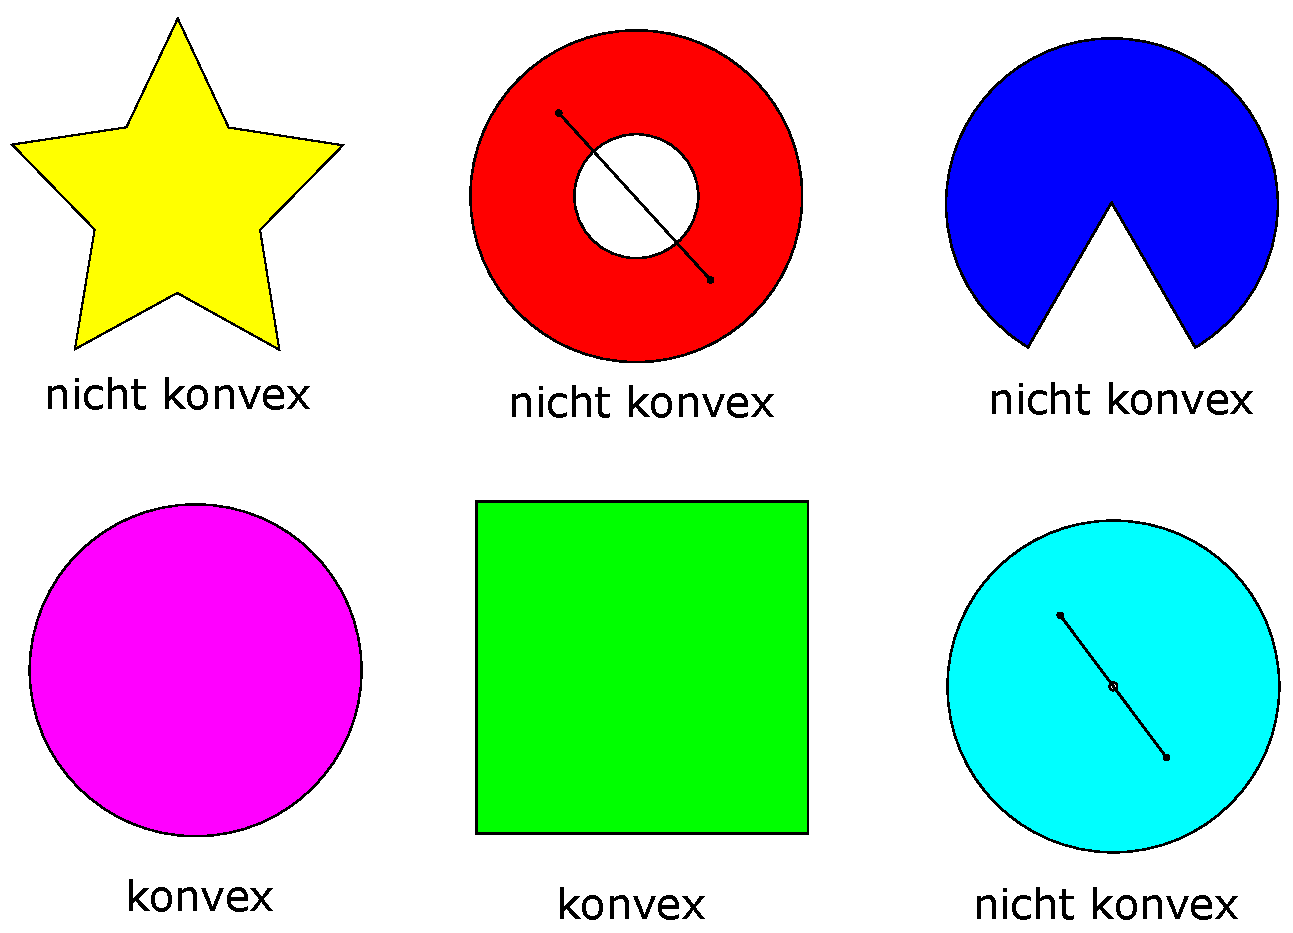
\includegraphics[width=0.40\textwidth]{konvexe-mengen.pdf}
\caption{Geometrische Beispiele für konvexe Mengen}
\end{figure}


\begin{Def}[Konvexe Menge]

Eine Menge $X$ heißt konvex, falls für alle $x, y \in X$ und $\lambda \in \mathbb{R}$ und $\lambda \in [0,1]$ gilt:

\begin{equation}
\lambda x + (1 - \lambda) \in X
\end{equation}

\end{Def}

\subsubsection{Beispiele konvexer Mengen}

\paragraph{Kugel}

Ein Beispiel für eine konvexe Menge ist die Menge $S$ der Vektoren, die eine Kugel mit dem Radius $r = 1$, deren Mittelpunkt im Ursprung liegt, beschreibt:

\begin{equation*}
S = \{ \in \mathbb{R}^{n} | \|v\| \le 1\}
\end{equation*}

\paragraph{Quadrant}

Auch die Quadranten des kartesischen Koordinatensystems lassen sich durch eine konvexe Menge erfassen. So gilt z.~B. für den ersten Quadranten:

\begin{equation*}
L = \{ x \in \mathbb{R}^{n} | x_1 \ge 0, x_2 \ge 0, ..., x_n \ge 0\}
\end{equation*}

\paragraph{Eistüte}

Bei einer Eistüte bzw. einem quadratischen Kegel handelt es sich um ein weiteres Beispiel für eine konvexe Menge, sonfern für $x \in \mathbb{R}^{n-1}$, $t \in \mathbb{R}$ gilt:

\begin{equation*}
Q = \{(x, t) \in \mathbb{R}^{n} | \|x\|^{2} \le t\}
\end{equation*}

\paragraph{Box}

Die Menge von Vektoren im $\mathbb{R}$ bilden eine konvexe Menge in Form einer Box mit der Seitenlänge 2, deren Mittelpunkt im Ursprung liegt, wenn gilt:

\begin{equation*}
B = \{x \ in \mathbb{R}^{n} | |x_{i}| \le 1, i = 1, ..., n\}
\end{equation*}

\subsection{Konvexe Programme}

Bei einem konvexen Programm handelt es sich um eine Funktion $f$ in Abhängigkeit vom Paramenter $x$. Im Rahmen der mathematischen Optimierung versuchen wir diese Funktion unter Berücksichtigung von Nebenbedingungen zu minimieren. Hierbei sind sowohl die Zielfunktion als auch die Menge der Punkte konvex.

\begin{Def}[Konvexes Programm]
Sei $f: \mathbb{R}^{n} \rightarrow \mathbb{R}$ eine konvexe Funktion und $X \subseteq \mathbb{R}^{n}$, so minimieren wir die Funktion $f(x)$ unter der Nebenbedigung, dass $x \in X$.
\end{Def}

% Bsp. 1

\subsection{Lineare Programme}

Lineare Programme lassen sich durch lineare Funktionen beschreiben, z.~B. $f(x) = \langle c, x \rangle$. Darüber hinaus sind eine lineare Abbildungsmatrix $A$, z.~B. $A = \begin{pmatrix}1 & 0 \\ 0 & 1 \end{pmatrix}$, sowie ein Vektor $b$ und ein weiterer Vektor $c$, z.~B. $c = \begin{pmatrix}1 \\ 0 \end{pmatrix}$, gegeben. $x$ ist dann zulässig, wenn $x \in X$ mit $X: Ax \le b$ bzw. $X = \{x \in \mathbb{R}^{n} | Ax \le b\}$ erfüllt ist. \\
So ergibt beispielsweise die Funktion $f(x)$:

\begin{equation*}
f(x) = \langle \begin{pmatrix}1 \\ 0 \end{pmatrix}, \begin{pmatrix}x_{1} \\ x_{2} \end{pmatrix} \rangle = x_{1}
\end{equation*}

Es folgt für die Nebenbedigungen:

\begin{equation*}
\begin{pmatrix}1 & 0 \\ 0 & 1 \end{pmatrix}
\end{equation*}

Hieraus folgt: $x_{1} \le 1$, $x_{2} \le 1$.

\subsection{Quadratische Programme}

Im Hinblick auf quadratische Programme verwenden wir dieselbe Herangehensweise. \\
Auch hier sei eine Funktion $f$ gegeben, z.~B. $f(x) = x^{T}Qx$ mit $Q = \begin{pmatrix}1 & 0 \\ 0 & 1 \end{pmatrix}$, die es zu unter der Bedingung $x \in X$ für $X: Ax \le b$ zu minmieren gilt.\\
Hieraus folgt:

\begin{align*}
f(x) &= x^{T}Qx \\
&= \begin{pmatrix}x_{1}, x_{2}\end{pmatrix} \begin{pmatrix}1 & 0 \\ 0 & 1\end{pmatrix} \begin{pmatrix}x_{1} \\ x_{2}\end{pmatrix} \\
&= \begin{pmatrix}x_{1}, x_{2}\end{pmatrix} \begin{pmatrix}x_{1} \\ x_{2}\end{pmatrix} \\
&= x_{1}^{2} + x_{2}^{2}
\end{align*}

